%----------------------------------------------------------------------------
\chapter{A rendszer részletes bemutatása} \label{chapter7}
%----------------------------------------------------------------------------

\section{Rendszer architektúra}

A rendszer architektúrája az alapfunkciót tekintve megváltozott. Minden \enquote{modul} egy közös Firebase adatbázisra csatlakozik, ahogy azt a ~\ref{fig:arch1} ábra is szemlélteti.

\begin{figure}[htbp]
	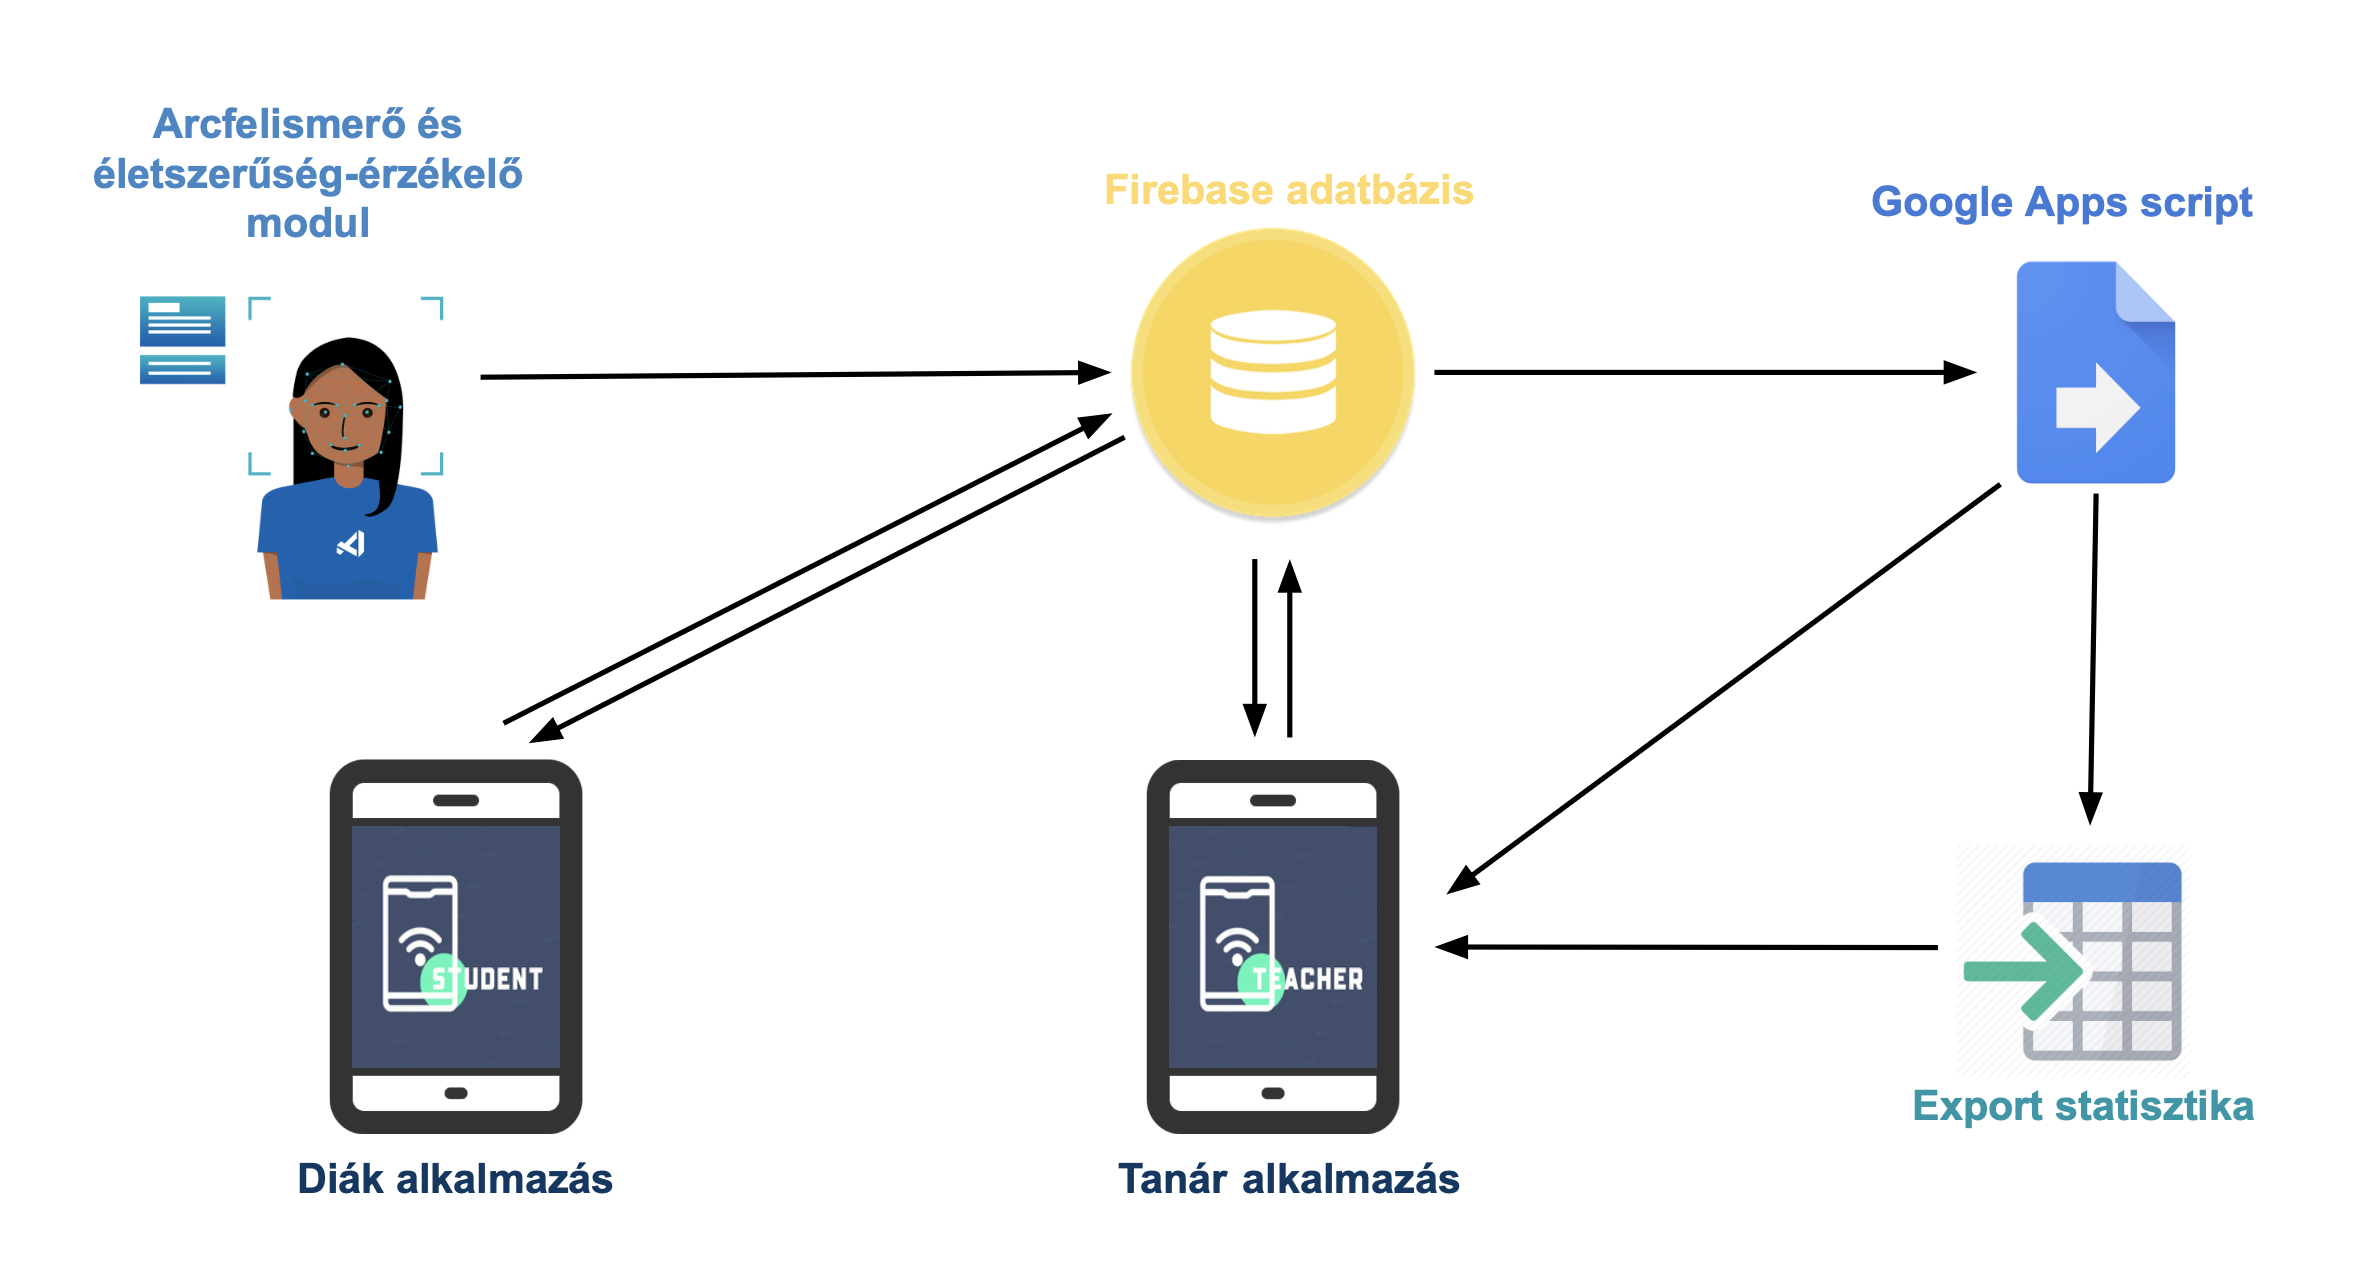
\includegraphics[width=\textwidth]{figures/architecture.png}
	\caption{A rendszer architektúrája}
	\label{fig:arch1}
\end{figure}

A rendszer a következő fő modulokból áll:

\begin{itemize}
    \item Arcfelismerő és életszerűség-érzékelő modul, amely felel a diákok azonosításáért, emellett szerepe a jelenlétek bevitele, valamint a diákok azonosításához szükséges előzőleges fényképek mentése is.
    \item Diák alkalmazás: fő feladata a jelenlétek megjelenítése a nyomon követhetőség elősegítése végett.
    \item Tanár alkalmazás: a jelenlétek megtekintése mellett fontos funkciója a jelenlétek kimentésének biztosítása különböző formátumokban.
    \item Google Apps script: ez teszi lehetővé a jelenlétek táblázatban való megjelenítését, amely az exporthoz szükségeltetik.
\end{itemize}


Amint az látható, architektúra szempontjából az arcfelismerő és életszerűség-érzékelő modulon kívül a rendszer többi része majdhogynem változatlan maradt, ennek okáért a továbbiakban csak az említett részt szeretném tárgyalni.


\paragraph{Arcfelismerő és életszerűség-érzékelő modul}\

Maga a jelenlétkezelő modul 3 kulcsfontosságú funkcióból áll:

\begin{itemize}
    \item Diákok fényképeinek mentése.
    \item Arcfelismerő funkció, ami a diák azonosításáért felel.
    \item Életszerűség-érzékelő algoritmus, amelynek az átjátszhatóság elleni védelemben van meghatározó szerepe.
\end{itemize}

\section{A diákok azonosítására használt fényképek mentése}

A hatékonyságot szem előtt tartva, a fényképek mentésére két megoldást próbáltunk ki.

Első megoldásként bővítettük a diákapplikáció funkcióit, méghozzá úgy, hogy a regisztrációkor az adatai mellett egy fotót is kell készítsen/feltöltsön magáról, amit a Firebase Storage-be mentettünk. Ezt a megközelítést bár lefejlesztettük, mégis eldobtuk két ok miatt. Egyrészt a diákot nem szeretnénk az applikáció használatára kényszeríteni. Ez azt jelenti, hogy csak akkor szükséges letöltenie, ha nyomon szeretné követni jelenléteit, illetve ha az app valamelyik másik funkcióját szeretné igénybe venni. Mivel a fénykép megléte kötelező jellegű, ezért láttuk jobbnak az alkalmazástól független megoldást keresni. A másik oka, miért nem ezt a megoldást választottuk az az, hogy nem szerettünk volna teljesen szabadkezet adni a fénykép milyensége végett a diáknak. Valamilyen szinten egységes fotókat szerettünk volna igényelni, éppen ezért döntöttünk úgy, hogy a fényképek készítése is az újonnan beépített modul feladata lesz. Ez azt jelenti, hogy a webkamera segítségével készül egy fotó a diákról, legelső órán, ezáltal mint minőségleg, mint pedig a \enquote{helyszínt} tekintve egységes képek fognak készülni.

A gyorsabb működés elérése érdekében egyelőre nem adatbázisba tároljuk a képeket, hanem lokálisan a jelenlétkezelő modult futtató gépen. Ez lehetővé teszi azt a megoldást is, hogy akár egy erre megbízott személy feltegye a diákok képeit tartalmazó mappát, amennyiben az egyetem rendelkezik vele.

\newpage

A fényképek mentésének kódbeli megvalósítását az alábbi kódrészlet szemlélteti:

\begin{lstlisting}[language=python]
if event == self.button_save:
    if values['class'] != "" and values['name'] != "" and values['neptun_id'] != "":
        cv2.imwrite('student-recognize-images/' + 
        values['neptun_id'] + "_" + 
        values['name'] + "_" + 
        values['class'] + '.png', frame)
        psg.popup('OK', 'Diak mentve!')
    else:
        psg.popup('Hiba', 'Minden mezo kitoltese kotelezo!')
\end{lstlisting}


\section{Diákok azonosítása: arcfelismerés}

Mivel előző megoldásunk, a QR kódos azonosítás, kijátszhatónak bizonyult, úgy döntöttünk, hogy a leggyakrabban alkalmazott biometrikus azonosítást, az arcfelismerést alkalmazzuk jelenlétkezelő rendszerünk alappilléreként.


A jelenlétek bevitelének elkezdését a mezők kitöltése után a kamera elindítása jelenti. Ezt követően megkapva az utolsó frame-et (\textit{get\_latest\_frame()}), két lista jön létre: az arcokat tartalmazó lista (\textit{face\_list}) és az életszerűség-érzékelés eredményét tartalmazó lista (\textit{live\_list}).

Ebben az alfejezetben az arcfelismerést fogom tárgyalni, melyet a \textit{face\_recognition\_process()} függvény biztosít. 

Az arcfelismerési procedúra lebonyolításához a Python \textit{Face Recognition} nevű könyvtárcsomagot használtuk. A dlib legmodernebb arcfelismerési funkciójával készült, mély tanulással.
A Dlib egy modern C++ eszközkészlet, amely gépi tanulási algoritmusokat és eszközöket tartalmaz komplex szoftverek létrehozásához C++ nyelven valós problémák megoldására. Az iparban és a tudományos életben egyaránt használják számos területen, beleértve a robotikát, a beágyazott eszközöket, a mobiltelefonokat és a nagy teljesítményű számítástechnikai környezeteket. A Dlib nyílt forráskódú licence lehetővé teszi, hogy bármilyen alkalmazásban ingyenesen használjuk.

A modell 99,38\%-os pontossággal rendelkezik a Labelled Faces in the Wild benchmarkon. A Labelled Faces in the Wild (LFW) arcfotók adatbázisa, amelyet a korlátlan arcfelismerés problémájának tanulmányozására terveztek.

A rendszer helyes működésének előfeltétele a diákok arcképeinek megléte. Ez az arcfelismerő modul működésének egyik kulcsfontosságú része, hiszen a meglévő képek szükségesek a megtalált arcok azonosításához.

Rendszerünk esetében, az elindítást követően szintén két listát hozunk létre: az első tartalmazza az arcok helyét (\textit{face\_locations(frame)}), azaz a talált arcok sorainak listáját téríti vissza (felső, jobb, alsó, bal) sorrendben. A második pedig az arcok kódolt értékét (\textit{face\_encodings(frame, face\_locations)}), ami alapvetően visszaadja s 128 dimenziós arckódolások listáját (a képen látható minden archoz egy). Ugyanarról a személyről készült két különböző képnek hasonló a kódolása, és két különböző embernek teljesen eltérő a kódolása.

Ezt követően végig iterálunk a listákon és egy összehasonlítást végzünk a kódolt arcok és a megtalált arc között, majd megnézzük, hogy mekkora az arcok közötti távolság, hogy egyezésnek tekintsük. A 0,6 tipikusan a legjobb teljesítmény (\textit{compare\_faces(known\_face\_encodings, face\_encoding, tolerance=0.6)}). A művelet során egy Igaz/Hamis listát kapunk, amely jelzi, hogy mely ismert arckódolások felelnek meg az ellenőrizendő arckódolásnak.

Mindezek után távolságot számítunk, \textit{face\_distance(known\_face\_encodings, face\_encoding)}, ahol adott arckódolások listája kerül összehasonlításra egy ismert arckódolással, és  minden összehasonlítandó arc esetén euklideszi távolságot kapunk.
A távolság megmutatja, mennyire hasonlóak az arcok. Ezután kiválasztásra kerül a legjobb értékű index, azaz ahol a távolság a legkisebb, ezt pedig az \textit{argmin(face\_distances)} függvény határozza meg, amely egy tengely mentén a minimális értékek indexeit adja vissza.

Az arcfelismerés megtörtént, társítjuk a megfelelő névvel, majd átadásra és megjelenítésre bocsájtjuk a feldolgozott információk adott részét.

Az arcfelismerő algoritmus során használt függvényt a \textit{face\_recognition} könyvtárcsomag biztosította.

A diákok azonosítására használt arcfelismerést lehetővétévő függvény kódrészlete itt látható: 

\begin{lstlisting}[language=python]
def face_recognition_process(self, image, scaling_factor=4):
        face_names, face_list = [], []

        image = cv2.resize(image, (0, 0), fx=1.0 /
                           scaling_factor, fy=1.0/scaling_factor)
        rgb_image = image[:, :, ::-1]

        face_locations = face_recognition.face_locations(rgb_image)
        face_encodings = face_recognition.face_encodings(rgb_image, face_locations)

        for face_encoding in face_encodings:
            matches = face_recognition.compare_faces(
                self.known_face_encodings, face_encoding, tolerance=0.6)
            face_distances = face_recognition.face_distance(
                self.known_face_encodings, face_encoding)
            best_match_index = np.argmin(face_distances)

            name = self.known_face_names[best_match_index] if matches[best_match_index] else "Unknown"
            face_names.append(name)

        for (top, right, bottom, left), name in zip(face_locations, face_names):
            top *= scaling_factor
            right *= scaling_factor
            bottom *= scaling_factor
            left *= scaling_factor

            face_list.append(FaceDetectionData(name, left, top, right, bottom))

        return face_list
\end{lstlisting}

\section{Biztonsági ellenőrzés: életszerűség-érzékelés}

Bizonyára az első gondolat a rendszer szemlélése során, hogy mi teszi biztonságosabbá az előző verzióval szemben, miért ne lehetne átverni azt egy másik eszközön megjelenített fotóval vagy viedóval. A válasz egyszerű: életszerűség-érzékelés. 
Annak érdekében, hogy az arcfelismerő rendszereket biztonságosabbá tegyük, képesnek kell lennünk a hamis/nem valódi arcok észlelésére – az ilyen algoritmusok esetén az életszerűség-érzékelés kifejezést használjuk.

Az életszerűség-detektor létrehozása érdekében egy mély neurális hálózatot tanítunk, amely képes megkülönböztetni a valódi és a hamis arcokat, és ezt a bináris osztályozók problémájaként kezelik ebben az esetben. Mivel a projekt során nem szerettünk volna ennek részletes hátterével foglalkozni, így egy előre betanított modellt használtunk a megvalósításhoz (\textit{liveness.model}).

Első lépésként betöltjük a meglévő arcdetektáló és életszerűség-érzékelő modellünket.
Mivel a Caffe (Convolutional Architecture for Fast Feature Embedding) használata mellett döntöttünk, a \textit{cv2.dnn.readNetFromCaffe} segítségével töltjük be a Caffe modelldefiníciós prototxt fájlját és az előre betanított modellünket a lemezről.

A Caffe egy mély tanulási keretrendszer, amely lehetővé teszi a felhasználók számára, hogy képosztályozási és képszegmentációs modelleket hozzanak létre. Kezdetben a felhasználók sima szöveges prototxt fájlként hozzák létre és mentik el a modelleiket. Miután a felhasználó betanította és finomítja modelljét a Caffe segítségével, a program elmenti a felhasználó által betanított modellt \textit{caffemodel} fájlként.

Ezt követően készítünk egy blob-ot a frame-ből, melynek mérete 300×300, hogy alkalmas legyen a Caffe arcdetektor használata esetén. Ezt átengedjük a hálón, hogy megkapjuk a detektálásokat és predikciókat.

Meghatározzuk a detektált arc koordinátáit, majd kivesszük az észlelt arc ROI-ját (Region Of Interest).

A predikció során megkapjuk a legnagyobb értéket, majd ezáltal meghatározunk egy score-t. Mivel nekünk is van egy előre megadott érték, ami fölött az arcot valódinak tekintjük, így összehasonlítást végezve megkapjuk a valós arcokat. Ellenben, ha ez a megkapott érték kisebb az általunk megadott küszöbértéknél, hamis arcnak tekintjük, amiket majd nem veszünk figyelembe a további műveletek végrehajtása során.

\newpage

Az életszerűség-észlelést az alábbi függvény írja le:

\begin{lstlisting}[language=python]
def live_detection_process(self, image):
        (h, w) = image.shape[:2]
        blob = cv2.dnn.blobFromImage(cv2.resize(image, (300, 300)),
                                     1.0,
                                     (300, 300),
                                     (104.0, 177.0, 123.0))

        self.net.setInput(blob)
        detections = self.net.forward()

        detection_list = []
        for i in range(0, detections.shape[2]):
            confidence = detections[0, 0, i, 2]

            if confidence > self.confidence:
                box = detections[0, 0, i, 3:7] * np.array([w, h, w, h])
                (startX, startY, endX, endY) = box.astype('int')

                startX = max(0, startX)
                startY = max(0, startY)
                endX = min(w, endX)
                endY = min(h, endY)

                face = image[startY:endY, startX:endX]
                face = cv2.resize(face, (32, 32))
                face = face.astype('float') / 255.0
                face = img_to_array(face)
                face = np.expand_dims(face, axis=0)
            
                predictions = self.model.predict(face)[0]
                max_index = np.argmax(predictions)
                score = predictions[max_index]

                if score > self.min_live_score and max_index == self.is_live:
                    detection_list.append(LiveDetectionData(
                        score, 'real', startX, startY, endX, endY))
                else:
                    detection_list.append(LiveDetectionData(
                        score, 'fake', startX, startY, endX, endY))
                        
        return detection_list
\end{lstlisting}

\newpage

\section{A jelenlét rögzítésének és a fénykép mentésének aktivitás diagramja}

Amint azt a ~\ref{fig:arch1} ábra (1) szemlélteti, a jelenétek bevitele az ábrázolt folyamat szerint megy végbe. A \textit{Kezdés} gomb megnyomásával elindul a detektálás. Amennyiben egy arc felismerésre kerül, azaz tudtuk azonosítani, az életszerűség-ellenőrzés veszi kezdetét. Ellenkező esetben nem történik azonosítás, csupán a felületen megjelenítjük az \textit{Unknown} címkét.

A következő lépésben az algoritmus el kell döntse, hogy élő arcot lát-e vagy sem. Amennyiben élő arcot érzékel, az azonosított diák jelenléte mentésre kerül az adatbázisba. Ellenkező esetben szintén nem történik semmilyen művelet, egy újabb címkével jelezzük, hogy az arc \enquote{hamis}.

A ~\ref{fig:arch1} ábra (2) mutatja be a fénykép mentésének folyamatát. Az alkalmazás indítása után, amennyiben az adott diák/diákok adatai még nem kerültek mentésre, az \textit{Új diák hozzáadása} lehetőséget választva ezt pótolni tudjuk. Ezt követően szükséges megadunk a kért adatokat, mint a szak, név és Neptun azonosító, és ezt követően tudjuk elkészíteni a fényképet, amit aztán lokálisan is lementünk.


\begin{figure}[htbp]
	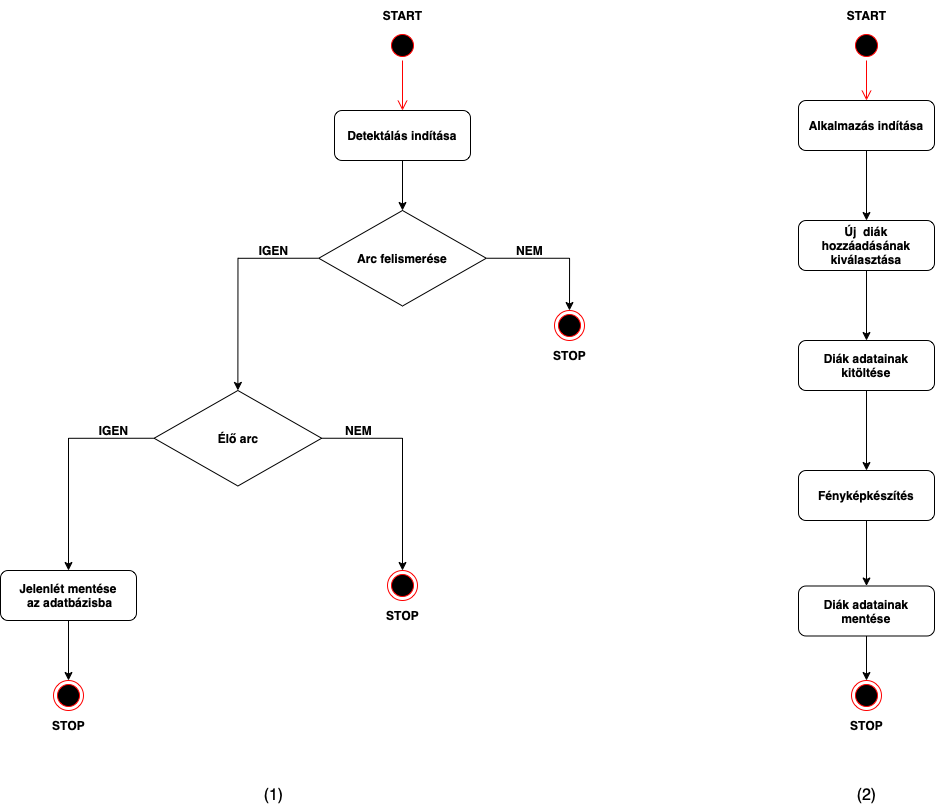
\includegraphics[width=15cm,height=12cm]{figures/activity11.png}
	\caption{A jelenlét rögzítésének (1) és a fénykép mentésének (2) aktivitás diagramja}
	\label{fig:activity1}
\end{figure}





